\documentclass{standalone}
\usepackage{tikz}
\usetikzlibrary{patterns, positioning}


\begin{document}
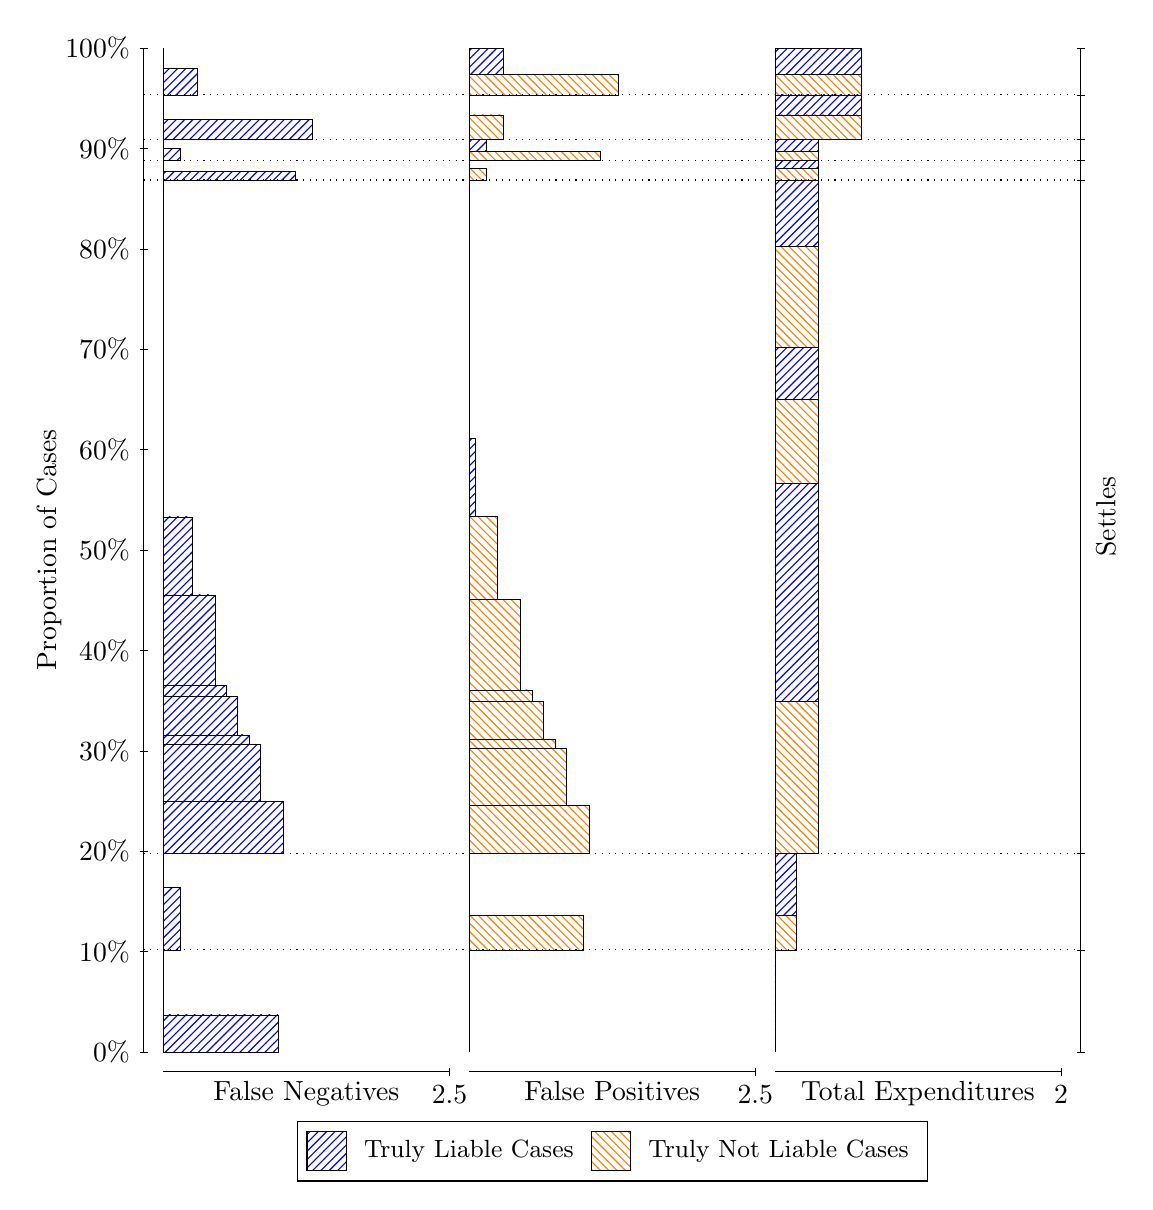
\begin{tikzpicture}
\draw[black, very thin] (1.5,1.75) -- (1.5,14.5);
\node[rotate=90, text=black, anchor=center] at (0.3, 8.125) {Proportion of Cases};
\draw[black, very thin] (1.45,1.75) -- (1.55,1.75);
\node[text=black, anchor=east] at (1.45, 1.75) {0\%};
\draw[black, very thin] (1.45,3.025) -- (1.55,3.025);
\node[text=black, anchor=east] at (1.45, 3.025) {10\%};
\draw[black, very thin] (1.45,4.3) -- (1.55,4.3);
\node[text=black, anchor=east] at (1.45, 4.3) {20\%};
\draw[black, very thin] (1.45,5.575) -- (1.55,5.575);
\node[text=black, anchor=east] at (1.45, 5.575) {30\%};
\draw[black, very thin] (1.45,6.85) -- (1.55,6.85);
\node[text=black, anchor=east] at (1.45, 6.85) {40\%};
\draw[black, very thin] (1.45,8.125) -- (1.55,8.125);
\node[text=black, anchor=east] at (1.45, 8.125) {50\%};
\draw[black, very thin] (1.45,9.4) -- (1.55,9.4);
\node[text=black, anchor=east] at (1.45, 9.4) {60\%};
\draw[black, very thin] (1.45,10.675) -- (1.55,10.675);
\node[text=black, anchor=east] at (1.45, 10.675) {70\%};
\draw[black, very thin] (1.45,11.95) -- (1.55,11.95);
\node[text=black, anchor=east] at (1.45, 11.95) {80\%};
\draw[black, very thin] (1.45,13.225) -- (1.55,13.225);
\node[text=black, anchor=east] at (1.45, 13.225) {90\%};
\draw[black, very thin] (1.45,14.5) -- (1.55,14.5);
\node[text=black, anchor=east] at (1.45, 14.5) {100\%};

\draw[black, very thin] (13.4,1.75) -- (13.4,14.5);
\draw[black, very thin] (13.35,1.75) -- (13.45,1.75);
\node[anchor=west] at (13.35, 1.75) {};
\draw[black, very thin] (13.35,3.0469) -- (13.45,3.0469);
\node[anchor=west] at (13.35, 3.0469) {};
\draw[black, very thin] (13.35,4.2752) -- (13.45,4.2752);
\node[anchor=west] at (13.35, 4.2752) {};
\draw[black, very thin] (13.35,12.824) -- (13.45,12.824);
\node[anchor=west] at (13.35, 12.824) {};
\draw[black, very thin] (13.35,13.074) -- (13.45,13.074);
\node[anchor=west] at (13.35, 13.074) {};
\draw[black, very thin] (13.35,13.337) -- (13.45,13.337);
\node[anchor=west] at (13.35, 13.337) {};
\draw[black, very thin] (13.35,13.905) -- (13.45,13.905);
\node[anchor=west] at (13.35, 13.905) {};
\draw[black, very thin] (13.35,14.5) -- (13.45,14.5);
\node[anchor=west] at (13.35, 14.5) {};

\draw[black, very thin, pattern color=blue, pattern=north east lines] (1.75,1.75) rectangle (3.2033,2.2207);
\draw[black, very thin, pattern color=orange, pattern=north west lines] (1.75,2.2207) rectangle (1.75,3.0469);
\draw[black, very thin, pattern color=blue, pattern=north east lines] (1.75,3.0469) rectangle (1.968,3.8371);
\draw[black, very thin, pattern color=orange, pattern=north west lines] (1.75,3.8371) rectangle (1.75,4.2752);
\draw[black, very thin, pattern color=blue, pattern=north east lines] (1.75,4.2752) rectangle (3.276,4.9354);
\draw[black, very thin, pattern color=blue, pattern=north east lines] (1.75,4.9354) rectangle (2.9853,5.661);
\draw[black, very thin, pattern color=blue, pattern=north east lines] (1.75,5.661) rectangle (2.84,5.777);
\draw[black, very thin, pattern color=blue, pattern=north east lines] (1.75,5.777) rectangle (2.6947,6.2662);
\draw[black, very thin, pattern color=blue, pattern=north east lines] (1.75,6.2662) rectangle (2.5493,6.408);
\draw[black, very thin, pattern color=blue, pattern=north east lines] (1.75,6.408) rectangle (2.404,7.5542);
\draw[black, very thin, pattern color=blue, pattern=north east lines] (1.75,7.5542) rectangle (2.1133,8.5457);
\draw[black, very thin, pattern color=orange, pattern=north west lines] (1.75,8.5457) rectangle (1.75,12.824);
\draw[black, very thin, pattern color=blue, pattern=north east lines] (1.75,12.824) rectangle (3.4213,12.93);
\draw[black, very thin, pattern color=orange, pattern=north west lines] (1.75,12.93) rectangle (1.75,13.074);
\draw[black, very thin, pattern color=blue, pattern=north east lines] (1.75,13.074) rectangle (1.968,13.225);
\draw[black, very thin, pattern color=orange, pattern=north west lines] (1.75,13.225) rectangle (1.75,13.337);
\draw[black, very thin, pattern color=blue, pattern=north east lines] (1.75,13.337) rectangle (3.6393,13.591);
\draw[black, very thin, pattern color=orange, pattern=north west lines] (1.75,13.591) rectangle (1.75,13.905);
\draw[black, very thin, pattern color=blue, pattern=north east lines] (1.75,13.905) rectangle (2.186,14.237);
\draw[black, very thin, pattern color=orange, pattern=north west lines] (1.75,14.237) rectangle (1.75,14.5);
\draw[black, very thin, pattern color=orange, pattern=north west lines] (5.6333,1.75) rectangle (5.6333,2.5762);
\draw[black, very thin, pattern color=blue, pattern=north east lines] (5.6333,2.5762) rectangle (5.6333,3.0469);
\draw[black, very thin, pattern color=orange, pattern=north west lines] (5.6333,3.0469) rectangle (7.0867,3.485);
\draw[black, very thin, pattern color=blue, pattern=north east lines] (5.6333,3.485) rectangle (5.6333,4.2752);
\draw[black, very thin, pattern color=orange, pattern=north west lines] (5.6333,4.2752) rectangle (7.1593,4.8779);
\draw[black, very thin, pattern color=orange, pattern=north west lines] (5.6333,4.8779) rectangle (6.8687,5.6034);
\draw[black, very thin, pattern color=orange, pattern=north west lines] (5.6333,5.6034) rectangle (6.7233,5.7195);
\draw[black, very thin, pattern color=orange, pattern=north west lines] (5.6333,5.7195) rectangle (6.578,6.2055);
\draw[black, very thin, pattern color=orange, pattern=north west lines] (5.6333,6.2055) rectangle (6.4327,6.3473);
\draw[black, very thin, pattern color=orange, pattern=north west lines] (5.6333,6.3473) rectangle (6.2873,7.4935);
\draw[black, very thin, pattern color=orange, pattern=north west lines] (5.6333,7.4935) rectangle (5.9967,8.5532);
\draw[black, very thin, pattern color=blue, pattern=north east lines] (5.6333,8.5532) rectangle (5.706,9.5446);
\draw[black, very thin, pattern color=blue, pattern=north east lines] (5.6333,9.5446) rectangle (5.6333,12.824);
\draw[black, very thin, pattern color=orange, pattern=north west lines] (5.6333,12.824) rectangle (5.8513,12.967);
\draw[black, very thin, pattern color=blue, pattern=north east lines] (5.6333,12.967) rectangle (5.6333,13.074);
\draw[black, very thin, pattern color=orange, pattern=north west lines] (5.6333,13.074) rectangle (7.3047,13.186);
\draw[black, very thin, pattern color=blue, pattern=north east lines] (5.6333,13.186) rectangle (5.8513,13.337);
\draw[black, very thin, pattern color=orange, pattern=north west lines] (5.6333,13.337) rectangle (6.0693,13.651);
\draw[black, very thin, pattern color=blue, pattern=north east lines] (5.6333,13.651) rectangle (5.6333,13.905);
\draw[black, very thin, pattern color=orange, pattern=north west lines] (5.6333,13.905) rectangle (7.5227,14.168);
\draw[black, very thin, pattern color=blue, pattern=north east lines] (5.6333,14.168) rectangle (6.0693,14.5);
\draw[black, very thin, pattern color=orange, pattern=north west lines] (9.5167,1.75) rectangle (9.5167,2.5762);
\draw[black, very thin, pattern color=blue, pattern=north east lines] (9.5167,2.5762) rectangle (9.5167,3.0469);
\draw[black, very thin, pattern color=orange, pattern=north west lines] (9.5167,3.0469) rectangle (9.7892,3.485);
\draw[black, very thin, pattern color=blue, pattern=north east lines] (9.5167,3.485) rectangle (9.7892,4.2752);
\draw[black, very thin, pattern color=orange, pattern=north west lines] (9.5167,4.2752) rectangle (10.062,6.2055);
\draw[black, very thin, pattern color=blue, pattern=north east lines] (9.5167,6.2055) rectangle (10.062,8.9741);
\draw[black, very thin, pattern color=orange, pattern=north west lines] (9.5167,8.9741) rectangle (10.062,10.034);
\draw[black, very thin, pattern color=blue, pattern=north east lines] (9.5167,10.034) rectangle (10.062,10.694);
\draw[black, very thin, pattern color=orange, pattern=north west lines] (9.5167,10.694) rectangle (10.062,11.982);
\draw[black, very thin, pattern color=blue, pattern=north east lines] (9.5167,11.982) rectangle (10.062,12.824);
\draw[black, very thin, pattern color=orange, pattern=north west lines] (9.5167,12.824) rectangle (10.062,12.967);
\draw[black, very thin, pattern color=blue, pattern=north east lines] (9.5167,12.967) rectangle (10.062,13.074);
\draw[black, very thin, pattern color=orange, pattern=north west lines] (9.5167,13.074) rectangle (10.062,13.186);
\draw[black, very thin, pattern color=blue, pattern=north east lines] (9.5167,13.186) rectangle (10.062,13.337);
\draw[black, very thin, pattern color=orange, pattern=north west lines] (9.5167,13.337) rectangle (10.607,13.651);
\draw[black, very thin, pattern color=blue, pattern=north east lines] (9.5167,13.651) rectangle (10.607,13.905);
\draw[black, very thin, pattern color=orange, pattern=north west lines] (9.5167,13.905) rectangle (10.607,14.168);
\draw[black, very thin, pattern color=blue, pattern=north east lines] (9.5167,14.168) rectangle (10.607,14.5);
\draw[black, dotted] (1.5,3.0469) -- (13.4,3.0469);
\draw[black, dotted] (1.5,4.2752) -- (13.4,4.2752);
\draw[black, dotted] (1.5,12.824) -- (13.4,12.824);
\draw[black, dotted] (1.5,13.074) -- (13.4,13.074);
\draw[black, dotted] (1.5,13.337) -- (13.4,13.337);
\draw[black, dotted] (1.5,13.905) -- (13.4,13.905);
\draw[black, very thin] (1.75,1.5) -- (5.3833,1.5);
\node[text=black, anchor=north] at (3.5667, 1.5) {False Negatives};
\draw[black, very thin] (5.3833,1.45) -- (5.3833,1.55);
\node[text=black, anchor=north] at (5.3833, 1.45) {2.5};

\draw[black, very thin] (5.6333,1.5) -- (9.2667,1.5);
\node[text=black, anchor=north] at (7.45, 1.5) {False Positives};
\draw[black, very thin] (9.2667,1.45) -- (9.2667,1.55);
\node[text=black, anchor=north] at (9.2667, 1.45) {2.5};

\draw[black, very thin] (9.5167,1.5) -- (13.15,1.5);
\node[text=black, anchor=north] at (11.333, 1.5) {Total Expenditures};
\draw[black, very thin] (13.15,1.45) -- (13.15,1.55);
\node[text=black, anchor=north] at (13.15, 1.45) {2};



\node[text=black, centered, rotate=90] at (13.72, 8.5494) {Settles};





\draw (7.449999999999999,1.5) node[draw=none] (baseCoordinate) {};
\begin{scope}[align=center]
        \matrix[scale=0.5, draw=black, below=0.5cm of baseCoordinate, nodes={draw}, column sep=0.1cm]{
            \node[rectangle, draw, minimum width=0.5cm, minimum height=0.5cm, pattern color=blue, pattern=north east lines] {}; &
            \node[draw=none, font=\small, text=black] (B) {Truly Liable Cases}; &
            \node[rectangle, draw, minimum width=0.5cm, minimum height=0.5cm, pattern color=orange, pattern=north west lines] {}; &
            \node[draw=none, font=\small, text=black] (B) {Truly Not Liable Cases}; \\
            };
\end{scope}

\end{tikzpicture}
\end{document}